\documentclass[aspectratio=169]{beamer}
\usetheme{Madrid}
\usecolortheme{default}
\usepackage{tikz}
\usetikzlibrary{calc,shapes,arrows.meta,positioning}

% --- Organization slides (TOC + section dividers) ---
\AtBeginSection[]
{
  \begin{frame}{Outline}
    \tableofcontents[currentsection]
  \end{frame}
}

\title{Lecture 4: AI Agents \& Tool Use}
\subtitle{Building an Application Routing Agent}
\author{University of Chicago}
\date{\today}

\begin{document}

\frame{\titlepage}

% Global outline
\begin{frame}{Outline}
  \tableofcontents
\end{frame}

\section{Where We Are and Where We're Going}

\begin{frame}{The Story So Far}
\textbf{Lecture 1}: Foundations
\begin{itemize}
    \item LLMs, tokens, context windows, APIs, pricing
\end{itemize}
\vspace{0.2cm}

\textbf{Lecture 2}: Building a System
\begin{itemize}
    \item Vertical slices and Crawl-Walk-Run
    \item Built a resume scorer: one prompt $\rightarrow$ one score
\end{itemize}
\vspace{0.2cm}

\textbf{Lecture 3}: Making It Good
\begin{itemize}
    \item Decomposition, citations, few-shot examples, temperature
    \item Improved the scorer until gold and silver resumes separate cleanly
\end{itemize}
\vspace{0.4cm}

\textbf{Result}: We have a reliable process for scoring resumes. \\
\textbf{Question}: Now what do we \textit{do} with those scores?
\end{frame}

\begin{frame}{What We Want to Build}
\textbf{A hiring pipeline doesn't end at a score.} After scoring, you need to:
\begin{itemize}
    \item Schedule interviews for strong candidates
    \item Reject poor matches with a polite email
    \item Flag edge cases for human review
    \item Route specialists to the right department
\end{itemize}
\vspace{0.3cm}

These are \textbf{actions}, not text. Our current system can't do any of them.
\vspace{0.3cm}

\textbf{Today}: Give LLMs the ability to \textit{act} --- through \textbf{tools} and \textbf{agents}.
\end{frame}

\section{The Optimized Scorer: What ``Solved'' Looks Like}

\begin{frame}{Recap: The Prompt That Works}
After three lectures of iteration, we have a scoring prompt with:
\vspace{0.2cm}
\begin{enumerate}
    \item \textbf{Core disqualifier checks} --- missing .NET $\rightarrow$ cap at 55, no SQL $\rightarrow$ cap at 60
    \item \textbf{Anchor-point scoring bands} --- explicit ranges (0--30, 31--49, \ldots, 93--100)
    \item \textbf{Bonus/penalty system} --- AWS +3, no Agile $-$2, frontend-only $-$10
    \item \textbf{7 calibration examples} --- from ``registered nurse $\rightarrow$ 5--15'' to ``9 years C\#/.NET + React + AWS $\rightarrow$ 93--97''
\end{enumerate}
\vspace{0.3cm}

This is context engineering in action: every rule, cap, and example is steering the model toward consistent, defensible scores.
\end{frame}

\begin{frame}{The Results}
\textbf{Scoring 8 resumes} (2 gold, 2 silver, 4 wild) with Mistral Small:
\vspace{0.3cm}

\begin{center}
\begin{tabular}{lcc}
\textbf{Tier} & \textbf{Scores} & \textbf{Mean} \\
\hline
Gold (strong match) & 97, 98 & 97.5 \\
Silver (weak match) & 72, 72 & 72.0 \\
Wild (random) & 10, 15, 15, 15 & 13.75 \\
\end{tabular}
\end{center}
\vspace{0.3cm}

\begin{itemize}
    \item Clean separation: gold $\gg$ silver $\gg$ wild
    \item Total cost: \$0.002 for all 8 resumes
    \item Uses a \textit{cheap} model (Mistral Small) --- the prompt does the heavy lifting
\end{itemize}
\vspace{0.3cm}

\textbf{Takeaway}: A well-engineered prompt can make even inexpensive models perform well. Now let's use these scores to \textit{take action}.
\end{frame}

\section{AI Agents}

\begin{frame}{What is an AI Agent?}
\begin{itemize}
    \item An \textbf{AI Agent} is an LLM that can use \textbf{tools} to interact with the outside world
    \item While a basic LLM can only generate text based on its training data, an agent can interact with ``tools" that:
\begin{itemize}
    \item \textbf{Database Tools}: Query databases, insert/update/delete records
    \item \textbf{API Tools}: Call REST APIs, interact with web services
    \item \textbf{File System Tools}: Read/write files, list directories
    \item \textbf{Code Execution Tools}: Run Python code, execute shell commands
    \item \textbf{Web Tools}: Search the web, scrape websites
    \item ...and more
\end{itemize}
\end{itemize}
\end{frame}


\begin{frame}{How Do They Work?}
\textbf{Agents are surprisingly simple}:
\vspace{0.3cm}

\begin{center}
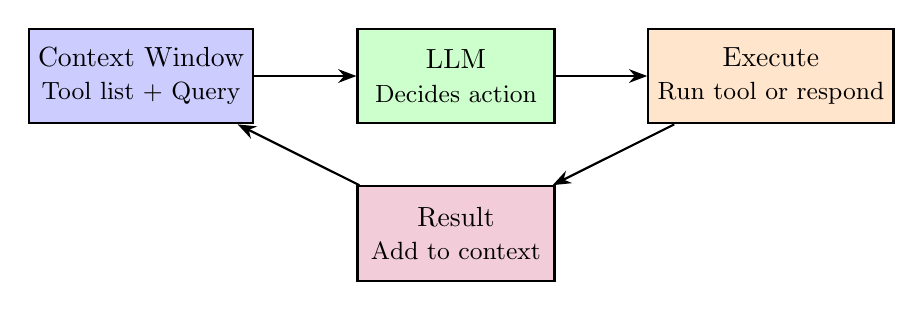
\begin{tikzpicture}[
  box/.style={rectangle, draw, thick, minimum width=2.5cm, minimum height=1.2cm, text centered, align=center},
  arrow/.style={->, thick, >=Stealth}
]
  \node[box, fill=blue!20] (context) at (0,0) {Context Window \\ {\small Tool list + Query}};
  \node[box, fill=green!20] (llm) at (4,0) {LLM \\ {\small Decides action}};
  \node[box, fill=orange!20] (execute) at (8,0) {Execute \\ {\small Run tool or respond}};
  \node[box, fill=purple!20] (result) at (4,-2) {Result \\ {\small Add to context}};

  \draw[arrow] (context) -- (llm);
  \draw[arrow] (llm) -- (execute);
  \draw[arrow] (execute) -- (result);
  \draw[arrow] (result) -- (context);
\end{tikzpicture}
\end{center}
\vspace{0.3cm}

\textbf{Key idea}: The LLM chooses which tool to use (or decides not to use any)
\end{frame}

\begin{frame}{The Agent Loop}
\begin{center}
We can simplify this into ``The Agent Loop"
\vspace{0.5cm}

\Large
Observe $\rightarrow$ Think $\rightarrow$ Act $\rightarrow$ Observe $\rightarrow$ \ldots
\end{center}
\vspace{0.8cm}
\begin{enumerate}
    \item \textbf{Observe}: Receive input (user query, tool results, system state)
    \item \textbf{Think}: Process information and decide what to do next
    \item \textbf{Act}: Execute actions (call tools, generate responses)
\end{enumerate}
\vspace{0.3cm}

\textbf{Each turn of the loop}:
\begin{enumerate}
    \item Agent sees: current state + what's been done so far
    \item Agent decides: which tool to call next (via LLM)
    \item Execute tool, log result
    \item Repeat until agent calls 'done' or max turns reached
\end{enumerate}
\end{frame}


\begin{frame}{Core Components of an Agent}
\textbf{Every agent system has four main components}:
\vspace{0.3cm}
\begin{enumerate}
    \item \textbf{System Prompt}
    \begin{itemize}
        \item Overall system parameters
    \end{itemize}

    \item \textbf{Tool Registry}
    \begin{itemize}
        \item Collection of available functions/tools with their descriptions and required parameters
        \item The agent may choose from this registry
    \end{itemize}

    \item \textbf{Action History / Conversation Memory}
    \begin{itemize}
        \item What tools have been called so far?
        \item What were the results?
    \end{itemize}

    \item \textbf{User Prompt / Task}
    \begin{itemize}
        \item The user-provided prompt
    \end{itemize}
\end{enumerate}
\end{frame}

\begin{frame}{The Tool Ecosystem}
\textbf{Different approaches for defining and sharing tools}:
\vspace{0.3cm}

\begin{itemize}
    \item \textbf{MCP (Model Context Protocol)}
    \begin{itemize}
        \item Standardized protocol for connecting AI assistants to external tools and data
        \item Developed by Anthropic; allows tools to be shared across different AI systems
        \item Example: Database connections, API integrations, file system access
    \end{itemize}
    \vspace{0.2cm}

    \item \textbf{agents.txt}
    \begin{itemize}
        \item Markdown file describing available tools and agent capabilities
        \item Simple, human-readable format for tool discovery
        \item Often placed in project root for documentation
    \end{itemize}
    \vspace{0.2cm}

    \item \textbf{Skills / Plugins}
    \begin{itemize}
        \item Pre-packaged tool collections for specific tasks
        \item Examples: PDF parsing, web scraping, git operations
        \item Can be installed and configured per-project
    \end{itemize}
\end{itemize}
\end{frame}


\begin{frame}{Example: Weather Query (Context)}
\textbf{Agent has access to a web search tool}
\vspace{0.2cm}

\textbf{User asks}: ``What's the weather tomorrow in Chicago?"
\vspace{0.3cm}

\textbf{Context window contains}:
\begin{itemize}
	

	\item \textbf{System Prompt:} 
    \begin{itemize}
        \item \texttt{Use the tools below to answer the user's query. Return your decision as JSON: \{"tool": ..., "parameters": \{...\}, "reasoning": "..."\}"}
	\end{itemize}
    \item \textbf{Tool Registry}:
    \begin{itemize}
        \item \texttt{web\_search(query: str) -> str}: Search the web and return results
        \item \texttt{done(message: str)}: Signal completion with a final message
    \end{itemize}
    \item \textbf{User Query}: ``What's the weather tomorrow in Chicago?"
\end{itemize}
\vspace{.3cm}
	\textbf{CODE sends this to LLM}
\end{frame}

\begin{frame}[fragile]{Example: Weather Query (Response)}
\textbf{LLM Response (Turn 1)}:
\vspace{0.2cm}

\begin{block}{JSON Output}
{\small
\begin{verbatim}
{
  "tool": "web_search",
  "parameters": {
    "query": "Chicago weather tomorrow forecast"
  },
  "reasoning": "Need to search for current weather
                forecast to answer the user's question"
}
\end{verbatim}
}
\end{block}
\vspace{0.3cm}

\end{frame}

\begin{frame}
	\textbf{CODE Response}:
\begin{enumerate}
    \item Parses this JSON
    \item Executes \texttt{web\_search("Chicago weather tomorrow forecast")}
    \item Gets result: ``Tomorrow: 45 deg F, partly cloudy, 20\% chance of rain"
    \item Adds result to context for next turn
\end{enumerate}

\end{frame}

\begin{frame}{Example: Weather Query (Turn 2)}
\textbf{Updated context window now includes}:
\begin{itemize}
    \item Original query
    \item Tool registry
    \item Previous action: Called \texttt{web\_search}
    \item Previous result: ``Tomorrow: 45 deg F, partly cloudy, 20\% chance of rain"
\end{itemize}
\vspace{0.3cm}
	\textbf{CODE Sends this to LLM}
\end{frame}

\begin{frame}[fragile]
	\textbf{LLM Response (Turn 2)}:
\begin{block}{JSON Output}

\begin{verbatim}
{
  "tool": "done",
  "parameters": {
    "message": "Tomorrow in Chicago will be 45 deg F with
                partly cloudy skies and a 20% chance of rain."
  },
  "reasoning": "I have the weather information needed
                to answer the user's question"
}
\end{verbatim}

\end{block}

\end{frame}

\begin{frame}[fragile]
	\textbf{CODE Response}

\begin{itemize}
	\item Since the tool is ``done", the code knows to stop the loop and return control to the user.
\end{itemize}
\end{frame}


\begin{frame}[fragile]{Implementing the Loop in Code}
\textbf{This is just a simple loop!}:
\vspace{0.2cm}

\begin{block}{Pseudo-code}
{\small
\begin{verbatim}
action_history = []
for turn in range(1, max_turns):
    decision = call_llm(context, tools, action_history)     # LLM 

    tool_name = decision['tool']
    params = decision['parameters']
    result = execute_tool(tool_name, params) # execute tool

    action_history.append({ 'tool': tool_name, 'result': result}) # update context

    if tool_name == 'done':     # Check if done
        break
\end{verbatim}
}
\end{block}
\end{frame}


\section{Readings}

\begin{frame}{Required Reading}
\textbf{Agents and Tools}
\begin{itemize}
    \item \href{https://www.anthropic.com/engineering/building-effective-agents}{Building Effective Agents} --- Anthropic's guide to agent patterns and best practices
\end{itemize}
\end{frame}

\begin{frame}{Reading Takeaway: Start Simple}
\textbf{Anthropic's \#1 finding}: The most successful agent deployments use simple, composable patterns --- not fancy frameworks.
\vspace{0.3cm}

\textbf{Their recommended progression}:
\begin{enumerate}
    \item Start with a single, well-engineered LLM call
    \item Add retrieval and structured output
    \item Only then consider multi-step agents
\end{enumerate}
\vspace{0.3cm}

\textbf{Sound familiar?}
\begin{itemize}
    \item Lecture 2: single prompt $\rightarrow$ score
    \item Lecture 3: decomposition, citations, few-shot
    \item Lecture 4 (today): agent loop with tools
\end{itemize}
\vspace{0.3cm}

You've been following best practice all along. Most real-world problems \textbf{don't need agents} --- a good prompt is enough.
\end{frame}

\begin{frame}{Reading Takeaway: Tool Design $>$ Prompt Design}
\textbf{Anthropic spent more time optimizing tools than prompts} on their coding agent.
\vspace{0.3cm}

Why? Because tools are the \textbf{interface} the model uses to act. Bad tool design $\rightarrow$ bad decisions.
\vspace{0.3cm}

\textbf{What makes a good tool?}
\begin{itemize}
    \item \textbf{Clear descriptions} --- would a new employee understand what this tool does?
    \item \textbf{Examples} in the tool description (edge cases, expected formats)
    \item \textbf{Obvious parameters} --- don't make the model guess
    \item \textbf{Error-proof design} --- when relative file paths caused bugs, they switched to absolute paths
\end{itemize}
\vspace{0.3cm}

\textbf{Lesson}: Treat tool descriptions like you treat prompts --- iterate, test, improve.
\end{frame}

\begin{frame}{Reading Takeaway: Ground Truth From the Environment}
\textbf{What makes agents different from a chain of prompts?}
\vspace{0.3cm}

Agents get \textbf{real information back} from tools that they didn't have before.
\vspace{0.3cm}

\begin{center}
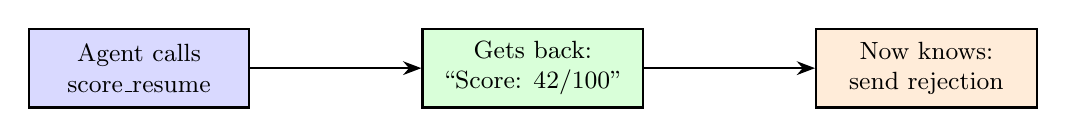
\begin{tikzpicture}[
  box/.style={rectangle, draw, thick, minimum width=2.8cm, minimum height=1cm, text centered, align=center, font=\small},
  arrow/.style={->, thick, >=Stealth}
]
  \node[box, fill=blue!15] (call) at (0,0) {Agent calls\\score\_resume};
  \node[box, fill=green!15] (result) at (5,0) {Gets back:\\``Score: 42/100''};
  \node[box, fill=orange!15] (decide) at (10,0) {Now knows:\\send rejection};
  \draw[arrow] (call) -- (result);
  \draw[arrow] (result) -- (decide);
\end{tikzpicture}
\end{center}
\vspace{0.3cm}

\begin{itemize}
    \item The agent \textbf{couldn't decide} on turn 1 --- it needed the score first
    \item The tool result \textbf{changed what happened next}
    \item This is why the loop exists: each step depends on what came before
\end{itemize}
\vspace{0.2cm}

Without this feedback, you just have a checklist --- not an agent.
\end{frame}

\section{Production Considerations}

\begin{frame}{Common Failure Modes}
\textbf{Agents can fail in predictable ways}:
\vspace{0.3cm}

\begin{enumerate}
    \item \textbf{Infinite Loops / Repeated Actions}
    \begin{itemize}
        \item Agent calls the same tool repeatedly without progress
        \item \textit{Mitigation}: Track action history, detect cycles, set max turns
    \end{itemize}
    \vspace{0.15cm}

    \item \textbf{Tool Hallucination}
    \begin{itemize}
        \item Agent invents tool names that don't exist in the registry
        \item \textit{Mitigation}: Validate tool names, provide clear error messages
    \end{itemize}
    \vspace{0.15cm}

    \item \textbf{Parameter Errors}
    \begin{itemize}
        \item Agent provides wrong types or missing required parameters
        \item \textit{Mitigation}: Schema validation, examples in tool descriptions
    \end{itemize}
    \vspace{0.15cm}

    \item \textbf{Premature Completion}
    \begin{itemize}
        \item Agent calls 'done' before completing necessary actions
        \item \textit{Mitigation}: Clear instructions about required steps, validate state
    \end{itemize}
\end{enumerate}
\end{frame}

\begin{frame}{Ralph Wiggum: Preventing Premature Completion}

\textbf{A viral tool for preventing premature completion}
\vspace{0.3cm}

\begin{center}
\includegraphics[width=0.85\textwidth]{images/RalphWiggum.png}
\end{center}

\vspace{0.3cm}
\footnotesize Source: \url{https://github.com/anthropics/claude-code/tree/main/plugins/ralph-wiggum}
\end{frame}


\begin{frame}{Real-World and Ethical Considerations}
\textbf{Agents act in the world --- that raises the stakes.}
\vspace{0.2cm}

\begin{columns}[T]
\begin{column}{0.48\textwidth}
\textbf{Engineering}
\begin{itemize}
    \item \textbf{Safety}: Max turn limits, cost caps, emergency stops
    \item \textbf{Observability}: Log every tool call, track costs, monitor success rates
    \item \textbf{Reliability}: Validate parameters, retry on transient errors, fall back to humans
\end{itemize}
\end{column}

\begin{column}{0.48\textwidth}
\textbf{Ethics}
\begin{itemize}
    \item \textbf{Bias}: Agents perpetuate training data biases --- resume screening can disadvantage demographics
    \item \textbf{Transparency}: Decisions must be explainable to stakeholders
    \item \textbf{Accountability}: Who is responsible when the agent is wrong?
\end{itemize}
\end{column}
\end{columns}

\vspace{0.4cm}
\textbf{The common answer: human-in-the-loop}
\begin{itemize}
    \item Design explicit ``flag for review'' tools for high-stakes, edge-case, or low-confidence decisions
    \item Keep an audit trail of every action and why it was taken
\end{itemize}
\end{frame}


\section{Agentic Email Outreach}

\begin{frame}{Agentic Resume Outreach}
\textbf{An agentic system that scores resumes and drafts personalized emails}
\begin{itemize}
	\item Tools make \textbf{real LLM calls} --- the agent genuinely needs the loop
	\item Agent can't draft the email until it knows the score
	\item Each tool creates new information that flows into the next decision
\end{itemize}
\vspace{0.3cm}

\end{frame}

\begin{frame}{Components}

\begin{enumerate}
    \item \textbf{Tool Registry} --- Python functions the agent can call
    \begin{itemize}
        \item \texttt{score\_resume} --- runs the L3 optimized scorer (real LLM call)
        \item \texttt{draft\_outreach\_email} --- generates a personalized email (real LLM call)
        \item \texttt{done} --- signals processing is complete
    \end{itemize}
    \vspace{0.2cm}

    \item \textbf{Agent Loop} --- Multi-turn decision making
    \begin{itemize}
        \item Observe action history
        \item Decide which tool to call next
        \item Execute tool and log result
        \item Repeat until done
    \end{itemize}
    \vspace{0.2cm}

    \item \textbf{Routing Rules}
    \begin{itemize}
        \item Score $\geq$ 80 $\rightarrow$ INTERVIEW
        \item Score 40--79 $\rightarrow$ REVIEW
        \item Score $<$ 40 $\rightarrow$ REJECT
    \end{itemize}
\end{enumerate}
\end{frame}


\begin{frame}[fragile]{Tool Example: score\_resume}
\textbf{A tool is a Python function that makes a real LLM call}
\vspace{0.2cm}

\begin{block}{Python Code}
{\small
\begin{verbatim}
def score_resume(candidate_id):
    """Score a candidate's resume. Returns score
    (0-100) and reasoning."""
    result = structured_llm_call(
        api_key=OPENROUTER_API_KEY,
        prompt=scoring_prompt,
        context_data={"resume": resume_text},
        output_schema={"score": "integer 0-100",
                       "reasoning": "1-3 sentences"},
        model=MODEL,
    )
    return {"status": "success",
            "score": result['result']['score'],
            "message": f"Score: {score}/100"}
\end{verbatim}
}
\end{block}

\end{frame}

\begin{frame}{Tool Registry}
\begin{itemize}
	\item The \textbf{Tool Registry} is a Python dictionary passed to the agent
	\item The LLM sees what tools are available and decides which to call
	\item Each entry contains:

\begin{itemize}
    \item \textbf{function}: the callable Python function
    \item \textbf{description}: what the tool does (used in the agent prompt)
    \item \textbf{parameters}: expected inputs
\end{itemize}

    \vspace{0.2cm}
    \item You define the tools --- \texttt{agent\_utils.py} provides the loop machinery
\end{itemize}
\end{frame}

\begin{frame}{Example Agent Flow}
\textbf{Candidate}: 7 years C\#/.NET, React, SQL Server
\vspace{0.3cm}

\textbf{Turn 1}:
\begin{itemize}
    \item Observe: No actions taken yet
    \item Decide: \texttt{score\_resume}
    \item Execute: Score 88/100 --- strong .NET/React/SQL match
\end{itemize}

\textbf{Turn 2}:
\begin{itemize}
    \item Observe: Score is 88 $\rightarrow$ INTERVIEW
    \item Decide: \texttt{draft\_outreach\_email}(outcome=INTERVIEW)
    \item Execute: Personalized interview invite drafted (312 chars)
\end{itemize}

\textbf{Turn 3}:
\begin{itemize}
    \item Observe: Score and email both complete
    \item Decide: \texttt{done}
    \item Execute: Processing complete
\end{itemize}
\end{frame}

\section{Your Turn: Building the Agent}

\begin{frame}{Today's Workflow}


\begin{center}
\textbf{You will build an email outreach agent}:
\vspace{0.3cm}
\Large
Open the notebook: \\[0.3cm]
\texttt{lecture\_4\_application\_routing\_agent.ipynb}
\\[1cm]

Define 3 tools (score, email, done) \\[0.3cm]
Run the agent loop and watch it work \\[0.3cm]
Read and compare the drafted emails \\[0.3cm]
Submit to the leaderboard
\end{center}
\end{frame}

\end{document}

